\begin{figure}[H]
	\centering
	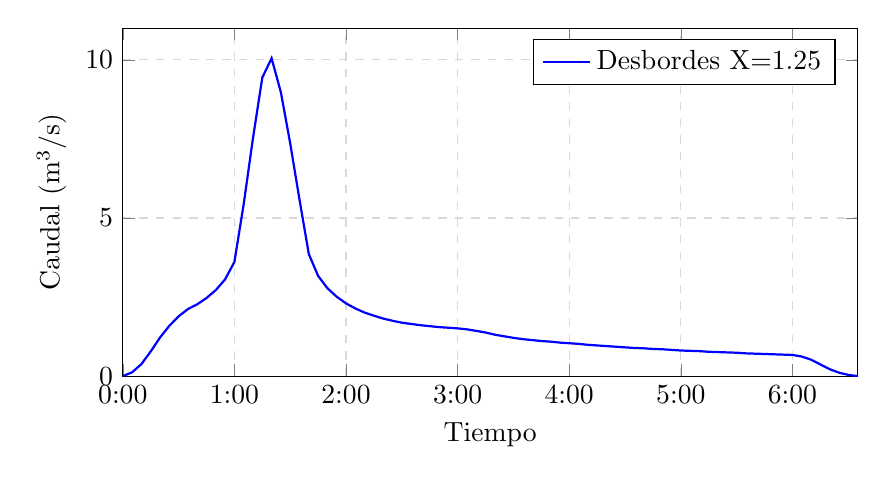
\begin{tikzpicture}
		\begin{axis}[
			width=0.9\textwidth,
			height=6cm,
			xlabel={Tiempo},
			ylabel={Caudal (m$^3$/s)},
			xmin=0,
			xmax=395,
			ymin=0,
			ymax=11,
			grid=major,
			grid style={dashed, gray!30},
			legend pos=north east,
			xtick={0, 60, 120, 180, 240, 300, 360},
			xticklabels={0:00, 1:00, 2:00, 3:00, 4:00, 5:00, 6:00},
			]
		% Desbordes X=1.25
		\addplot [
		blue,
		thick,
		solid,
		] coordinates {
				(0, 0.00) (5, 0.12) (10, 0.38) (15, 0.78) (20, 1.22)
				(25, 1.59) (30, 1.89) (35, 2.12) (40, 2.27) (45, 2.47)
				(50, 2.72) (55, 3.06) (60, 3.61) (65, 5.44) (70, 7.53)
				(75, 9.44) (80, 10.05) (85, 8.97) (90, 7.36) (95, 5.58)
				(100, 3.86) (105, 3.17) (110, 2.78) (115, 2.51) (120, 2.30)
				(125, 2.14) (130, 2.01) (135, 1.91) (140, 1.82) (145, 1.75)
				(150, 1.69) (155, 1.65) (160, 1.61) (165, 1.58) (170, 1.55)
				(175, 1.53) (180, 1.51) (185, 1.48) (190, 1.43) (195, 1.38)
				(200, 1.31) (205, 1.26) (210, 1.21) (215, 1.17) (220, 1.14)
				(225, 1.11) (230, 1.09) (235, 1.06) (240, 1.04) (245, 1.02)
				(250, 0.99) (255, 0.97) (260, 0.95) (265, 0.93) (270, 0.91)
				(275, 0.89) (280, 0.88) (285, 0.86) (290, 0.85) (295, 0.83)
				(300, 0.81) (305, 0.80) (310, 0.79) (315, 0.77) (320, 0.76)
				(325, 0.75) (330, 0.74) (335, 0.72) (340, 0.71) (345, 0.70)
				(350, 0.69) (355, 0.68) (360, 0.67) (365, 0.62) (370, 0.52)
				(375, 0.37) (380, 0.22) (385, 0.11) (390, 0.04) (395, 0.00)
		};
		\addlegendentry{Desbordes X=1.25}

		\end{axis}
	\end{tikzpicture}
	\caption{Hidrograma - Desbordes + GZ $T_r$=10 años ($Q_p$=10.048 m$^3$/s)}
	\label{fig:hydro_desbordes_gz_Tr10_X125}
\end{figure}
